\documentclass[12pt,letter]{article}
\usepackage{../downey_format}




\begin{document}
	
%	\large{}
%	
%	\title{\vspace{-2cm} Chapter 1: Basic concepts of Control Theory}
%	\date{}
%	\maketitle

	% set the section number, along with figure and equation numbers
	\setcounter{section}{6}	
	\setcounter{figure}{\thesection}   
	\renewcommand\thefigure{\thesection.\arabic{figure}}
	\setcounter{equation}{\thesection}   
	\renewcommand\theequation{\thesection.\arabic{equation}}

\section{Control Systems}

\subsection{On-Off (Bang-Bang) Control}

On-off (bang-bang) control is the most basic type of control system, operating by simply switching the output fully on or fully off in response to the measured variable. When the process value falls below a setpoint, the controller turns the system on; when it exceeds the setpoint, it turns it off. This approach is common in applications where precise control is not required, such as hot water heaters and HVAC systems, offering a simple, low-cost, and reliable method of maintaining conditions within an acceptable range.


\begin{figure}[H]
	\centering
	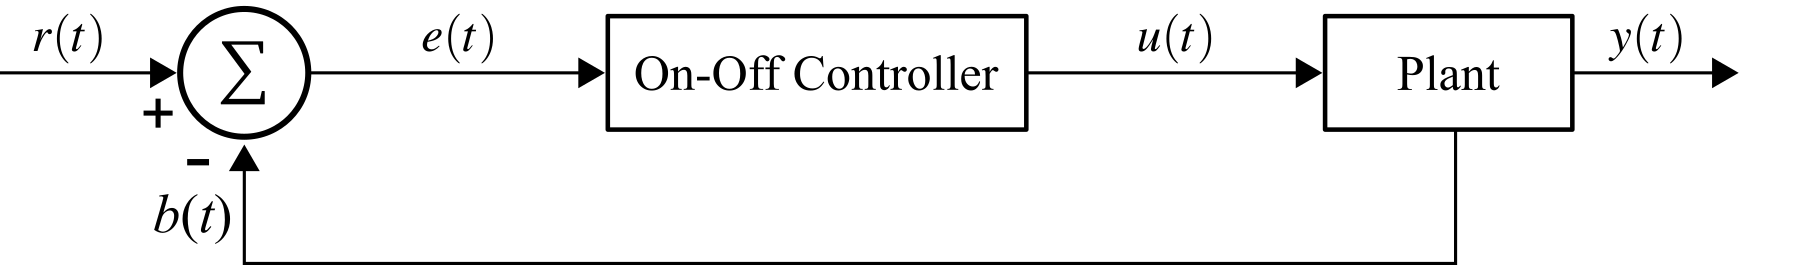
\includegraphics[]{../figures/controller_Bang-Bang.png}
	\caption{On-Off (Bang-Bang) controller for a system with feedback, where $r(t)$ is the desired setpoint (SP) and $y(t)$ is the measured process value (PV).}
	\label{fig:controller_Bang-Bang}
\end{figure}



\subsection{Proportional-Integral-Derivative (PID) Control}


Proportional-Integral-Derivative (PID) Control is a three-term controller that employs feedback that is widely used in continuous control systems, including for the control of structural systems. A PID controller seeks to minimize the measured error value $e(t)$ between a desired setpoint (SP) and a measured process variable (PV) by applying corrections based on the proportional ($P$), integral ($I$), and derivative ($D$) terms (denoted P, I, and D respectively), from which it gets its name.

\begin{figure}[H]
	\centering
	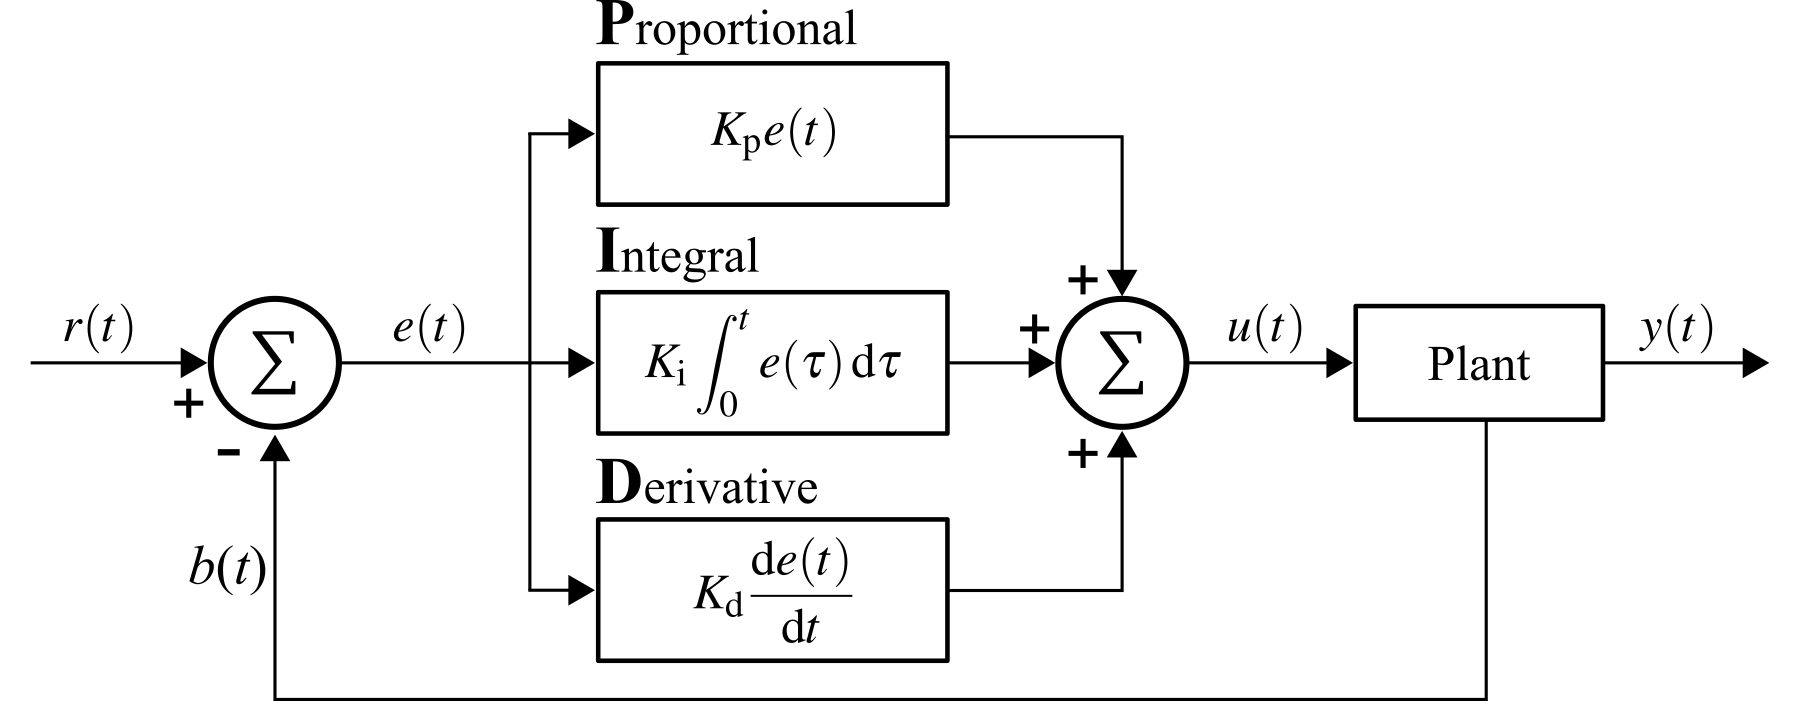
\includegraphics[]{../figures/controller_PID.png}
	\caption{Generalized PID controller for a system with feedback, where $r(t)$ is the desired setpoint (SP) and $y(t)$ is the measured process value (PV).}
	\label{fig:PID_controller}
\end{figure}





The overall control equation is defined as
\begin{equation}
	u(t) = K_\text{p} e(t) + K_\text{i} \int_0^t e(\tau) \,\mathrm{d}\tau + K_\text{d} \frac{\mathrm{d}e(t)}{\mathrm{d}t}
\end{equation}
where $K_\text{p}$, $K_\text{i}$, and $K_\text{d}$ are non-negative coefficients for the proportional, integral, and derivative terms, respectively. The PID controller is diagrammed in figure~\ref{fig:PID_controller} for a system with feedback control, such as that shown in figure~\ref{fig:active_vibration_control_FBD}. Moreover, in the Laplace-derived $s$ domain, the transfer function of the PID controller is defined as
\begin{equation}
	\Laplace{s} = K_\text{p} + \frac{K_\text{i}}{s} + K_\text{d}s
\end{equation}
where $s$ is the complex frequency. A temporal response for the 1-DOF shown in figure~\ref{fig:active_vibration_control_FBD} when controlled with a PID controller is reported in figure~\ref{fig:PID_temporal_response_1}.

\begin{figure}[H]
	\centering
	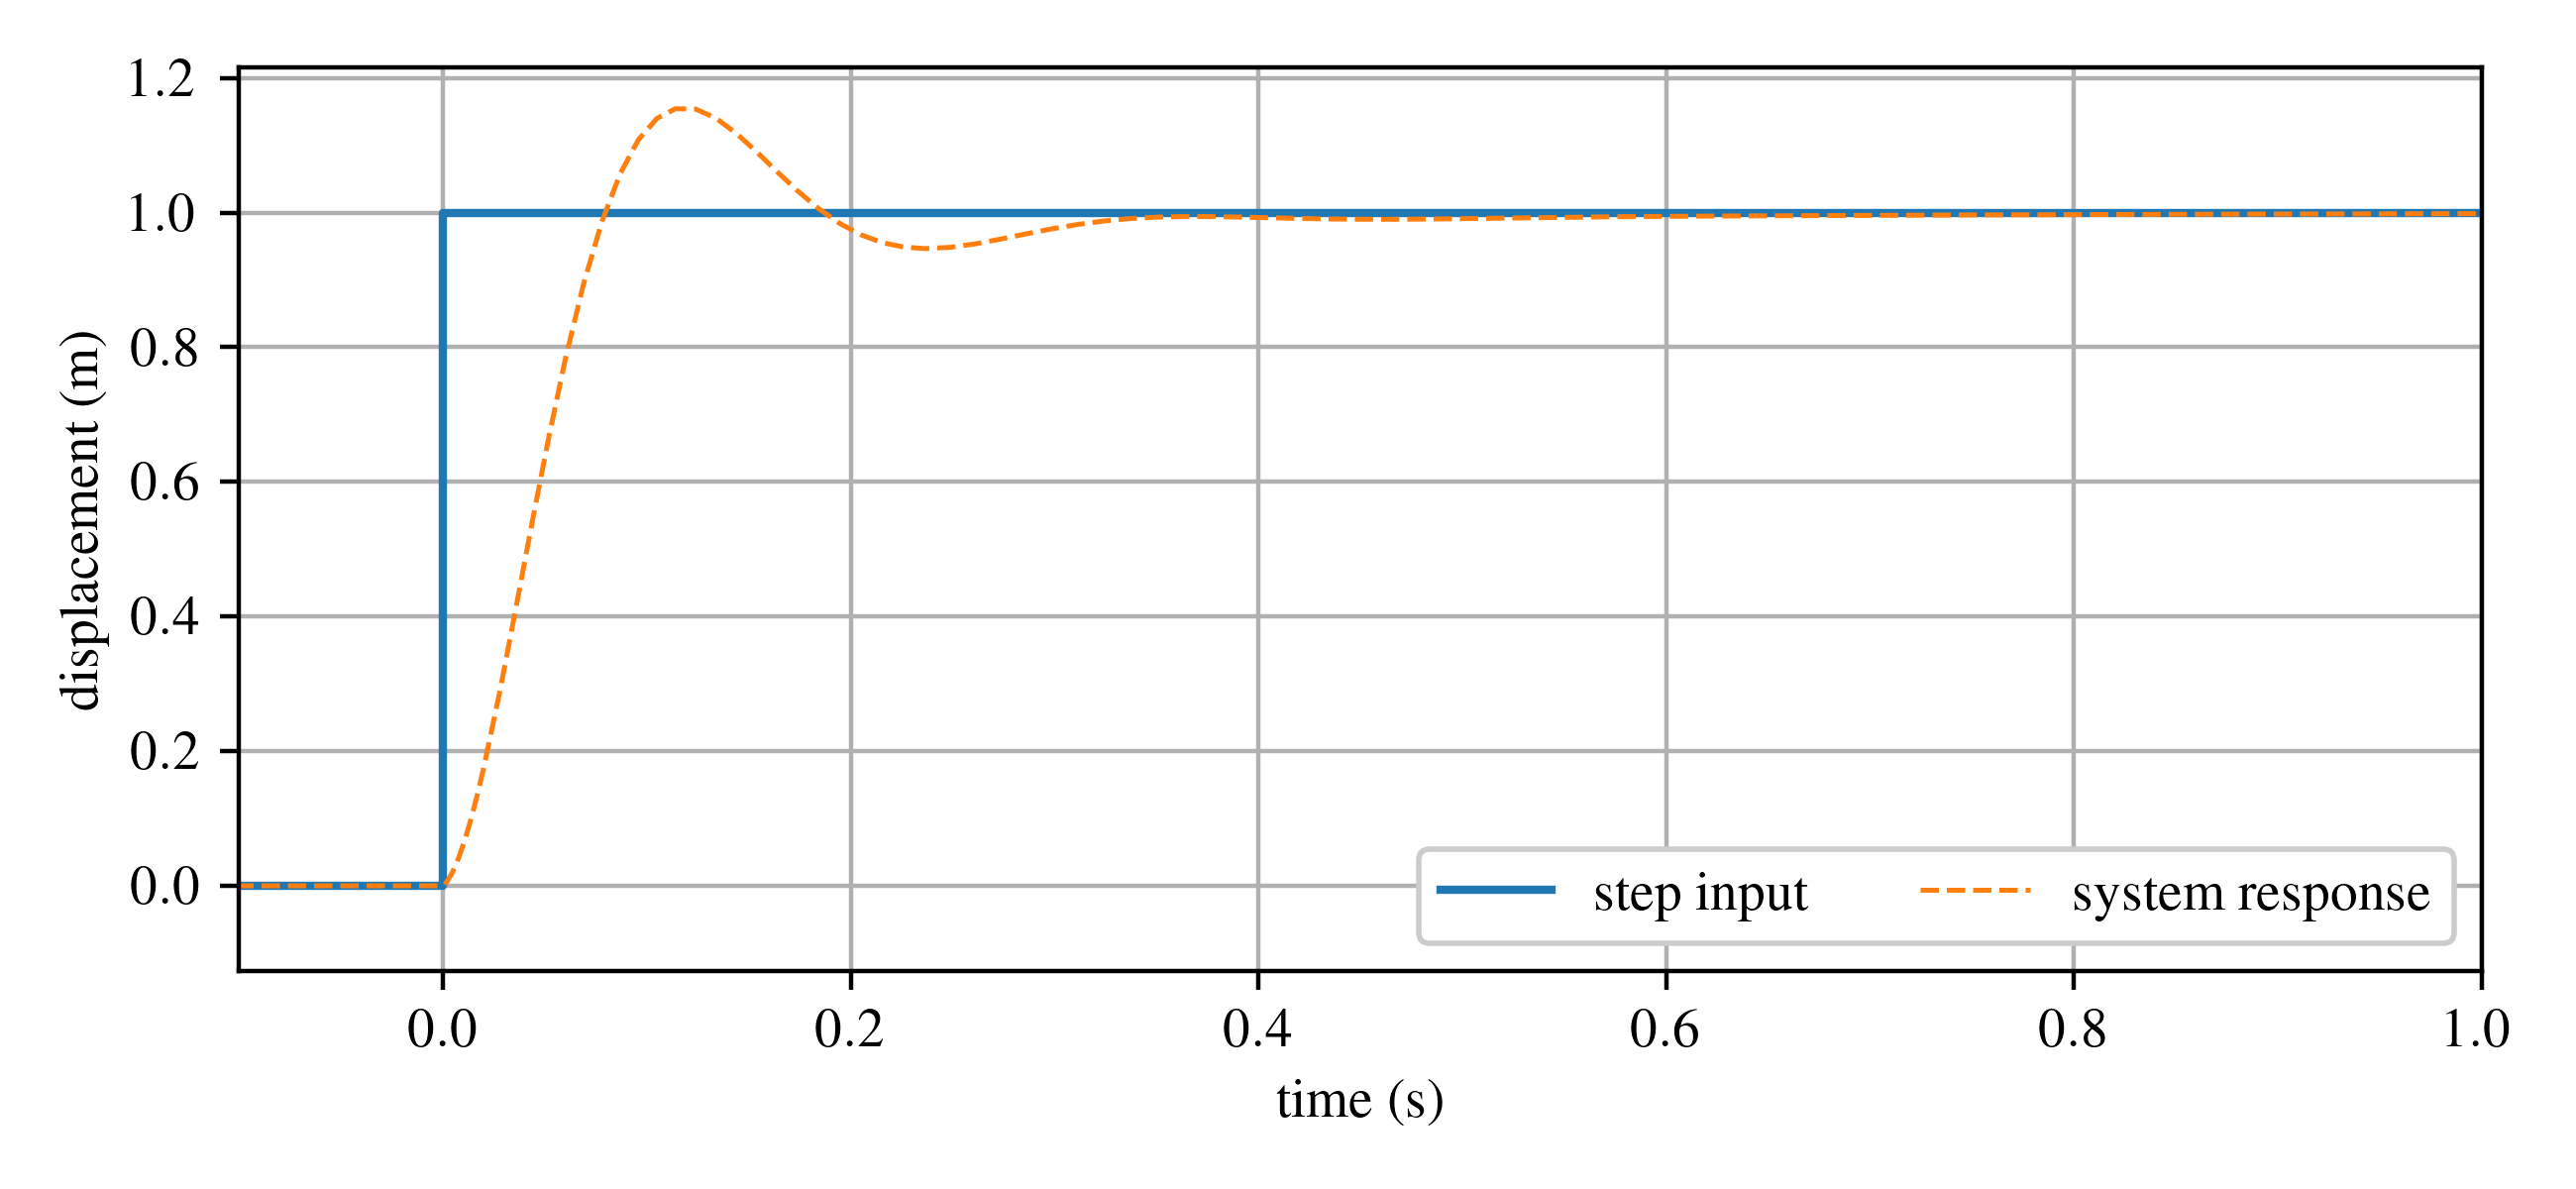
\includegraphics[]{../figures/PID_temporal_response_1.png}
	\caption{System response for a 1-DOF system controlled with a PID.}
	\label{fig:PID_temporal_response_1}
\end{figure}


\begin{figure}[H]
	\centering
	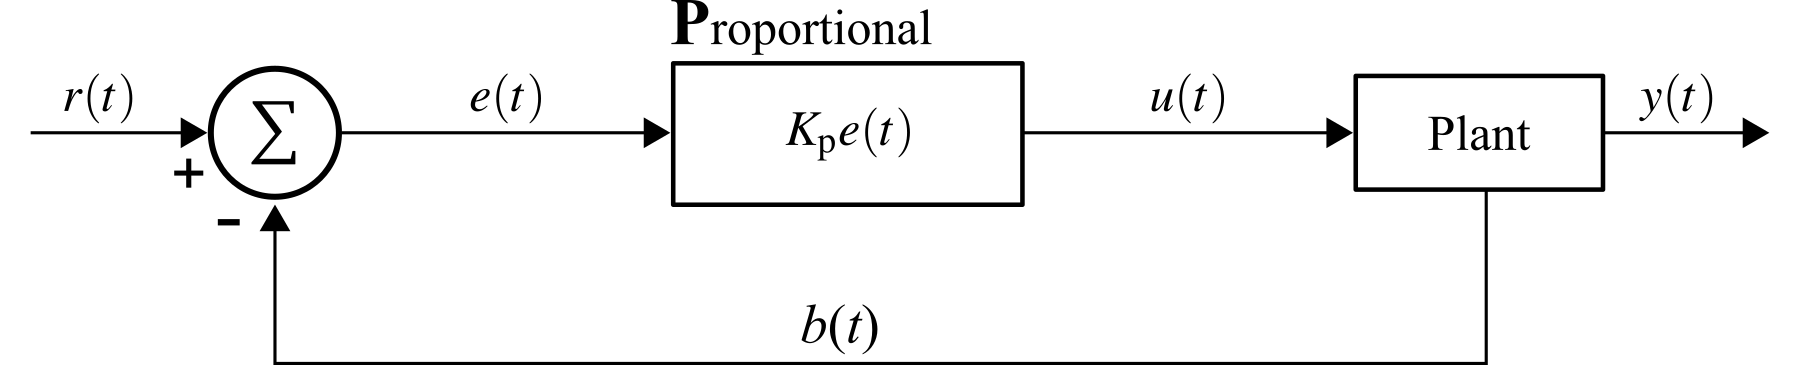
\includegraphics[]{../figures/controller_P.png}
	\caption{Generalized PID controller for a system with feedback, where $r(t)$ is the desired setpoint (SP) and $y(t)$ is the measured process value (PV).}
	\label{fig:P_controller}
\end{figure}


\begin{figure}[H]
	\centering
	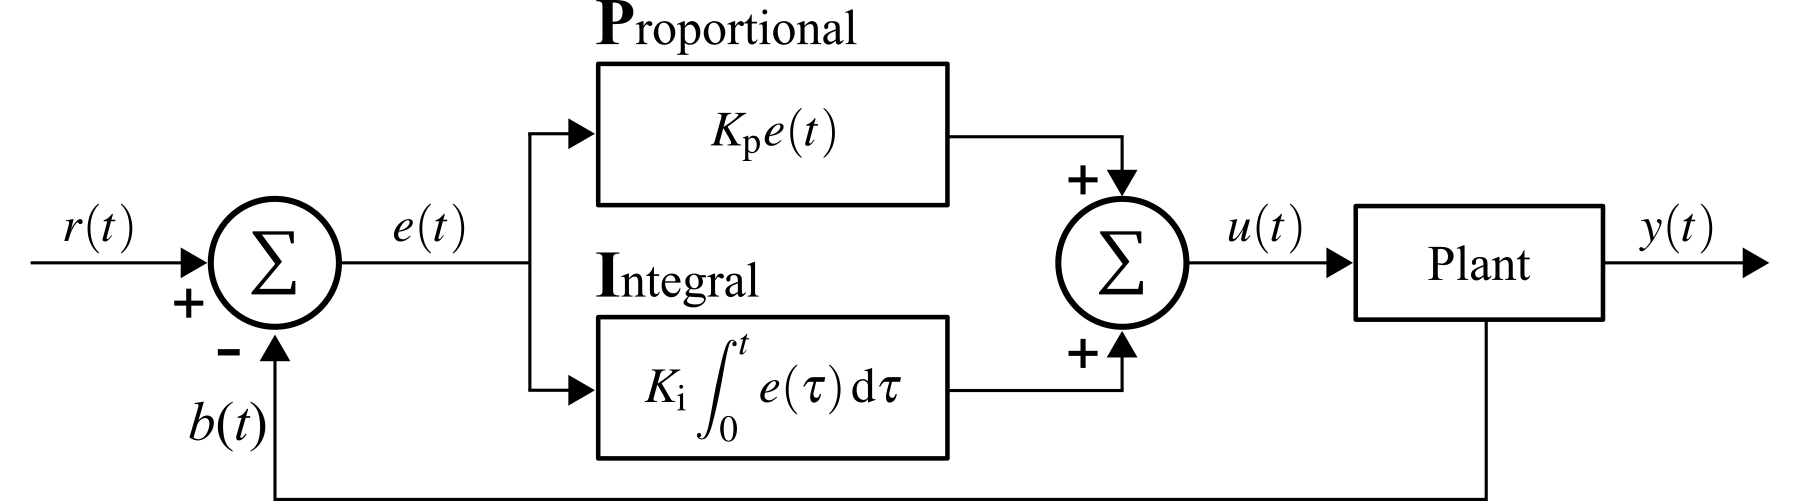
\includegraphics[]{../figures/controller_PI.png}
	\caption{Generalized PID controller for a system with feedback, where $r(t)$ is the desired setpoint (SP) and $y(t)$ is the measured process value (PV).}
	\label{fig:PI_controller}
\end{figure}


\begin{figure}[H]
	\centering
	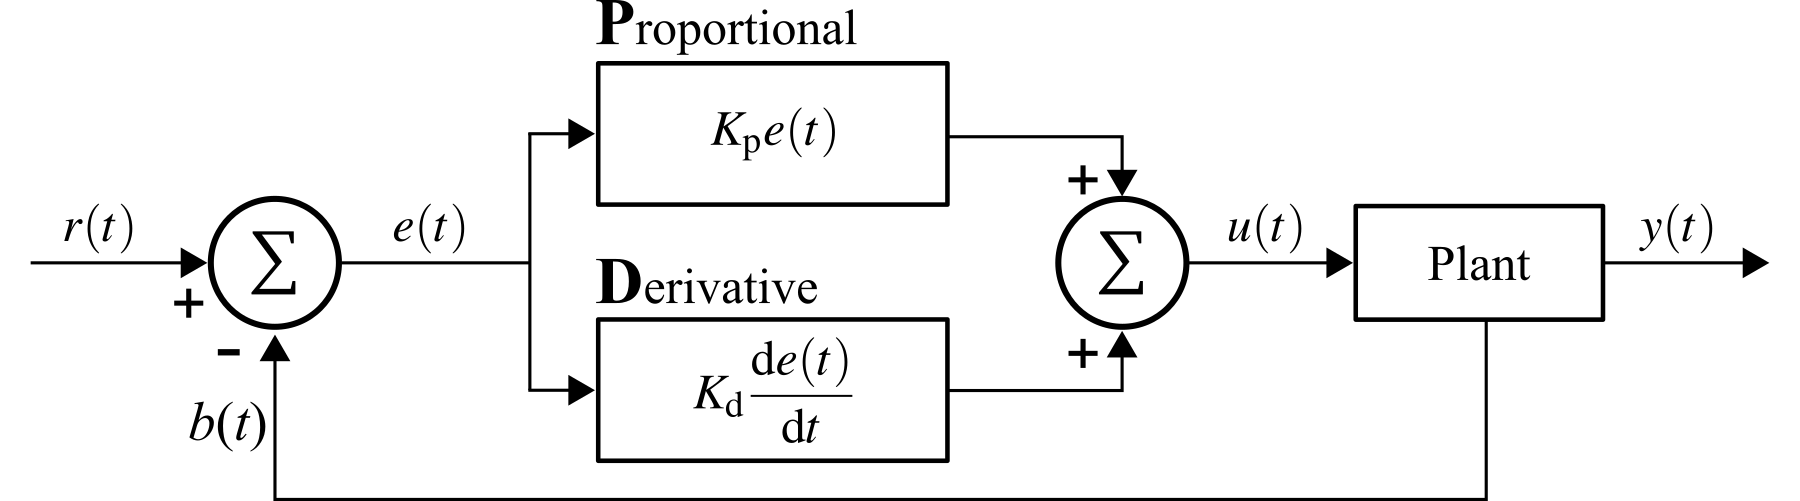
\includegraphics[]{../figures/controller_PD.png}
	\caption{Generalized PID controller for a system with feedback, where $r(t)$ is the desired setpoint (SP) and $y(t)$ is the measured process value (PV).}
	\label{fig:PD_controller}
\end{figure}



\begin{review}
	\label{sec:control_systems_review}

		\textbf{Nicolas Minorsky and the Need for Better Control}
	
		\noindent Continuous control systems have been widely used for centuries. For example, consider that the centrifugal governor which uses spinning weights was used by Christiaan Huygens in the 1600s in the Netherlands to regulate the gap between millstones in windmills or by James Watt who famously linked a stem regulator to a centrifugal governor to control steam turbines. 

		Arguably, the Russian American engineer Nicolas Minorsky was the first to develop the theoretical analysis for the three-term control we now call PID. This was done in 1922 while he was researching and designing automatic ship steering for the US Navy. He based his work on watching how a ship's helmsman responds to wave loading on a ship, with a delayed input to the helm that not only considered the current ship course but also past errors and the desired rate of change for the ship. For a helmsman, the goal is stability, not absolute control, which simplifies how one thinks about the challenge of control.
		
	\begin{figure}[H]
		\centering
		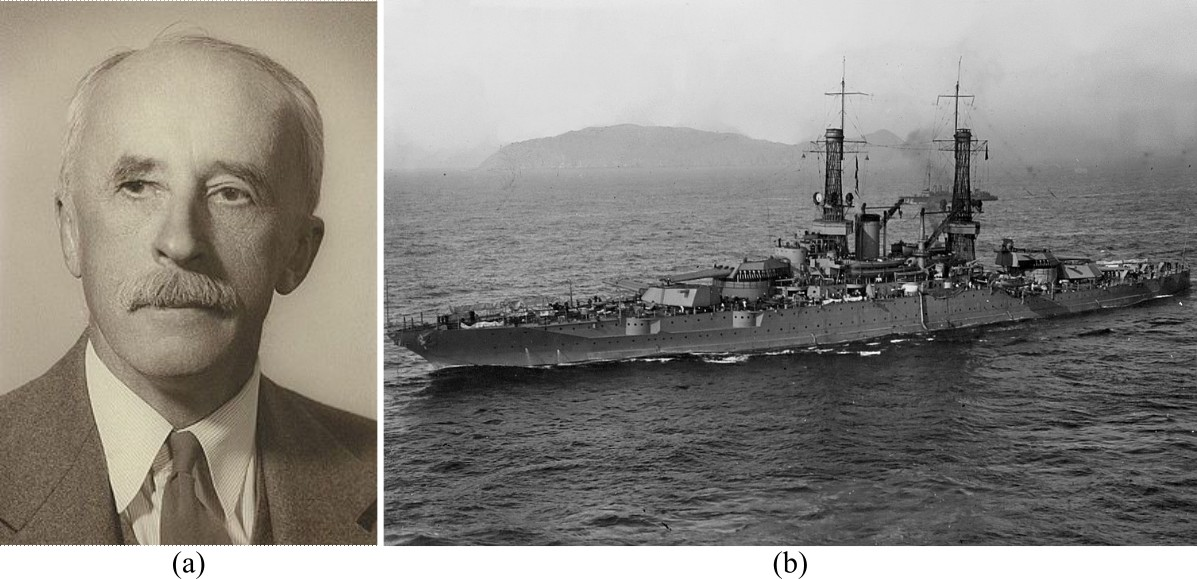
\includegraphics[width=6in]{../figures/PID_Nicolas_Minorsky_and_USS_New_Mexico}
		\caption{Historical perspective of PID control showing: (a) Portrait of Nicolas Minorsky \protect\footnotemark[1] and (b) the battleship USS New Mexico (BB-40) of the United States Navy which was the first to implement PID control in its steering \protect\footnotemark[2]. }
		\label{fig:PID_Nicolas_Minorsky_and_USS_New_Mexico}
	\end{figure}

	\footnotetext[1]{Peter Minorsky, grandson of Nicolas Minorsky, CC BY-SA 1.0 $<$https://creativecommons.org/licenses/by-sa/1.0$>$, via Wikimedia Commons} 
	\footnotetext[2]{U.S. Navy, Public domain, via Wikimedia Commons} 
	
\end{review}



\subsection{Control Systems}
\includepdf[pages=-,pagecommand={},width=0.9\textwidth]{PDF_notes/Control_Systems.pdf}

\subsection{Stability of feedback control systems and root locus}
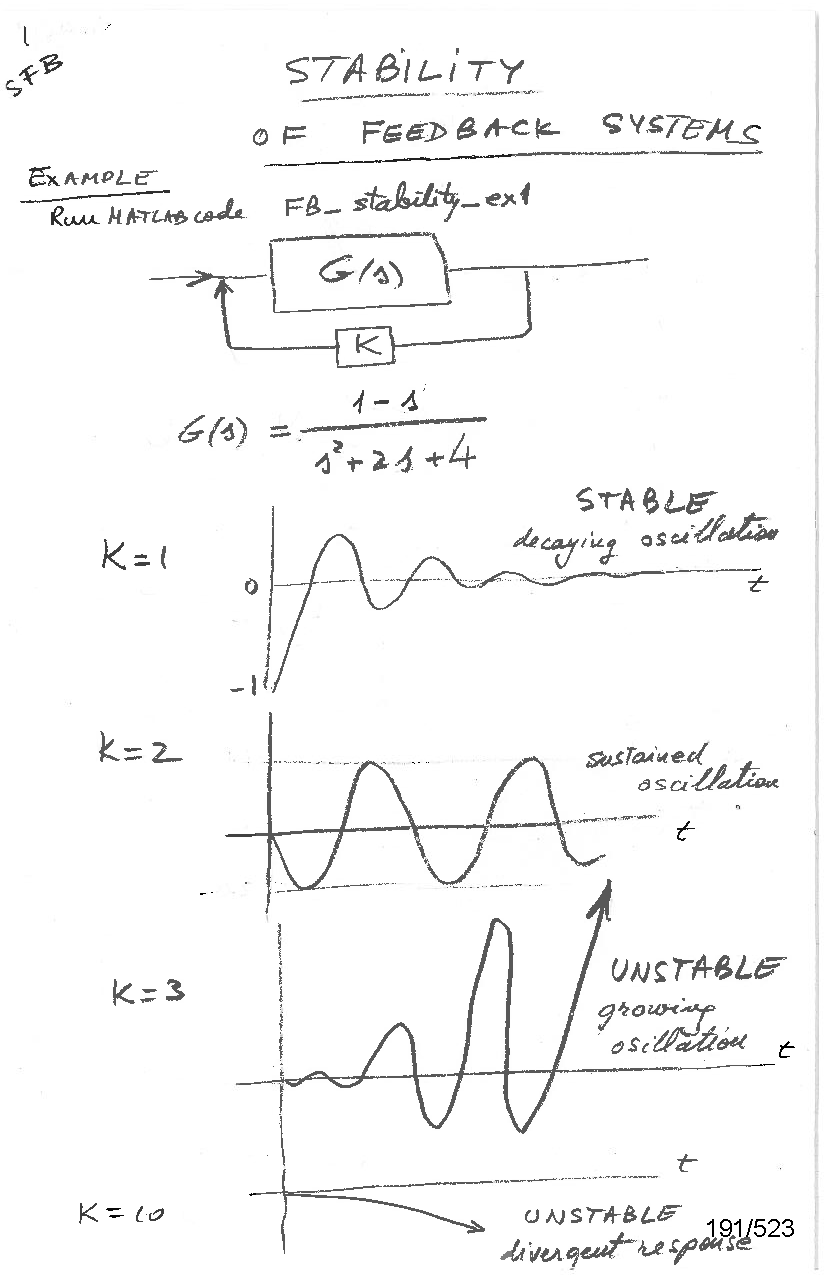
\includepdf[pages=-,pagecommand={},width=0.9\textwidth]{PDF_notes/Stability_of_feedback_control.pdf}

\subsection{Stability Criteria}
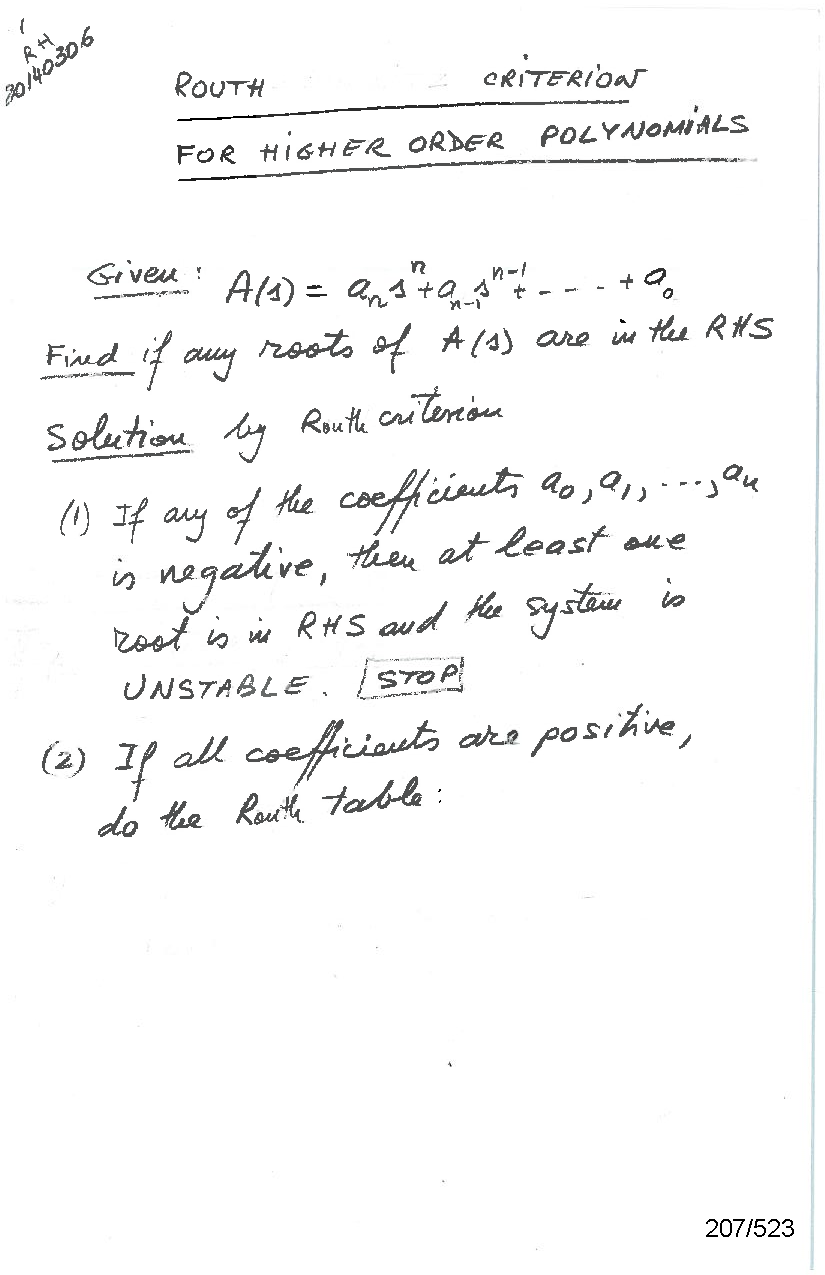
\includepdf[pages=-,pagecommand={},width=0.9\textwidth]{PDF_notes/Stability_Criteria.pdf}

\subsection{Feedback Controllers}
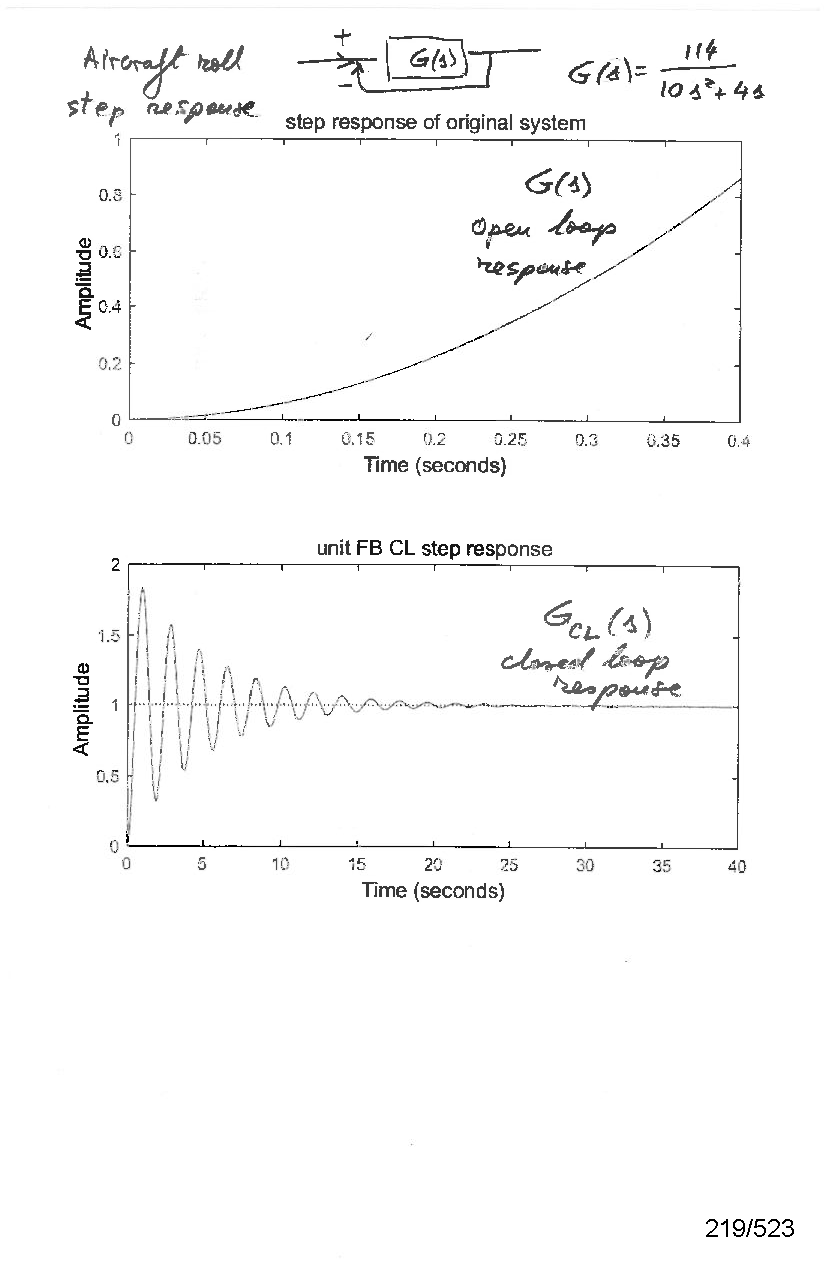
\includepdf[pages=-,pagecommand={},width=0.9\textwidth]{PDF_notes/Feedback_Controllers.pdf}

\subsection{SIMULINK Aircraft Roll Motion}
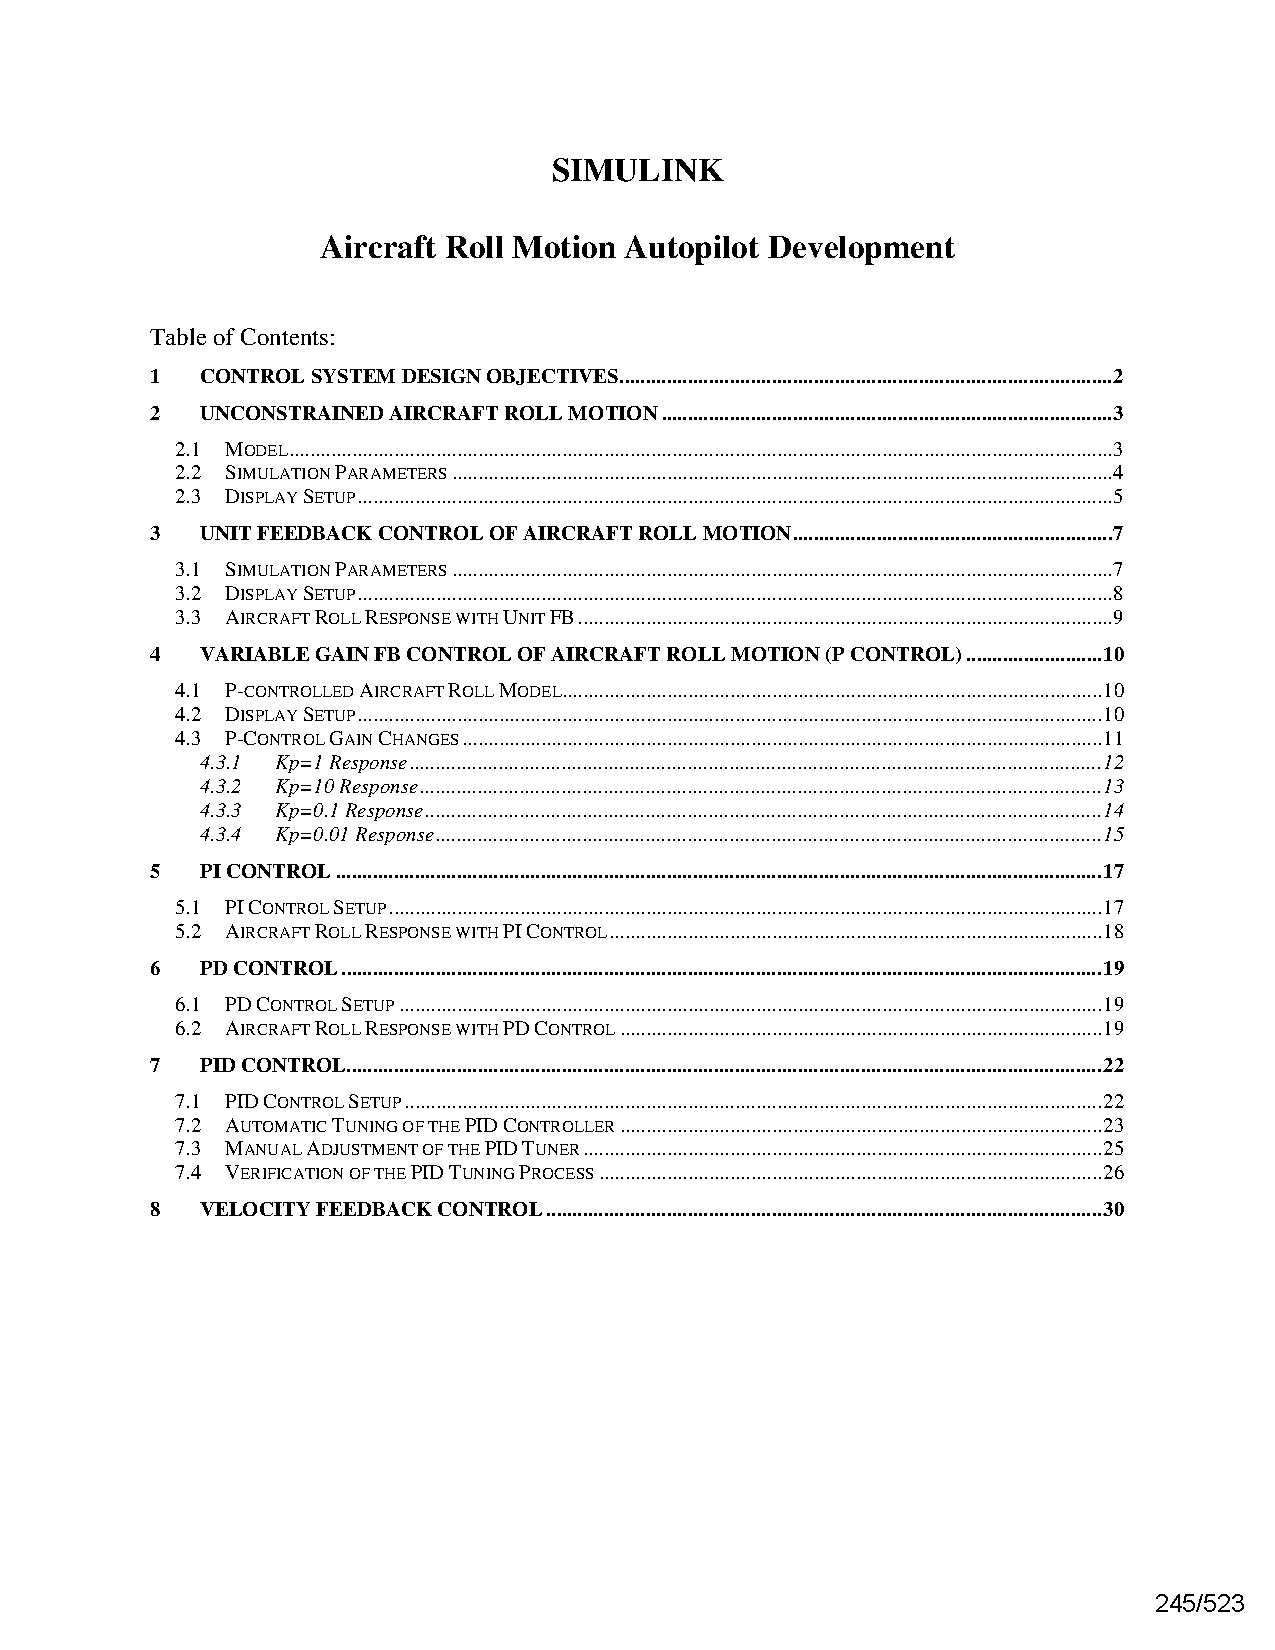
\includepdf[pages=-,pagecommand={},width=0.9\textwidth]{PDF_notes/SIMULINK_Aircraft_Roll_Motion.pdf}

\subsection{Feedback Controllers (continued)}
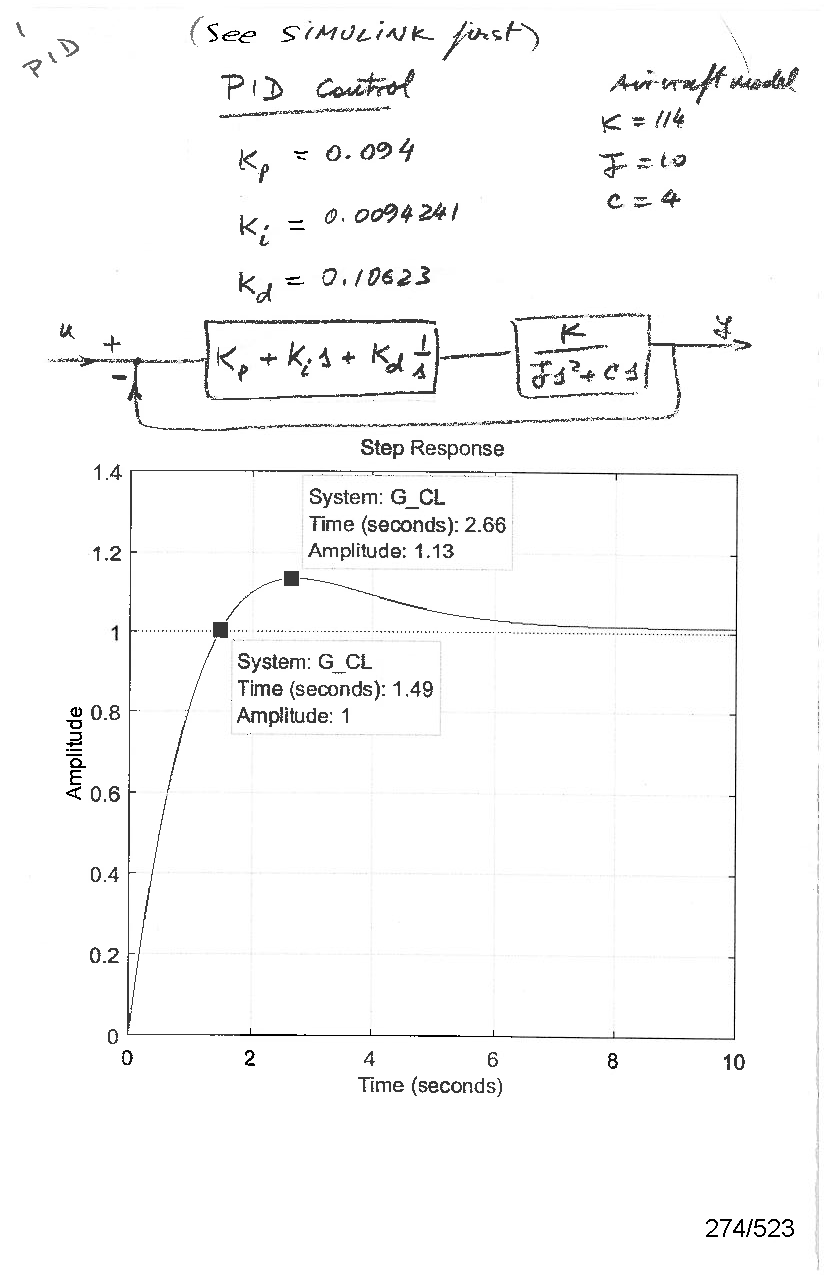
\includepdf[pages=-,pagecommand={},width=0.9\textwidth]{PDF_notes/Feedback_Controllers_continued.pdf}

\subsection{SIMULINK Aircraft Roll Motion (continued)}
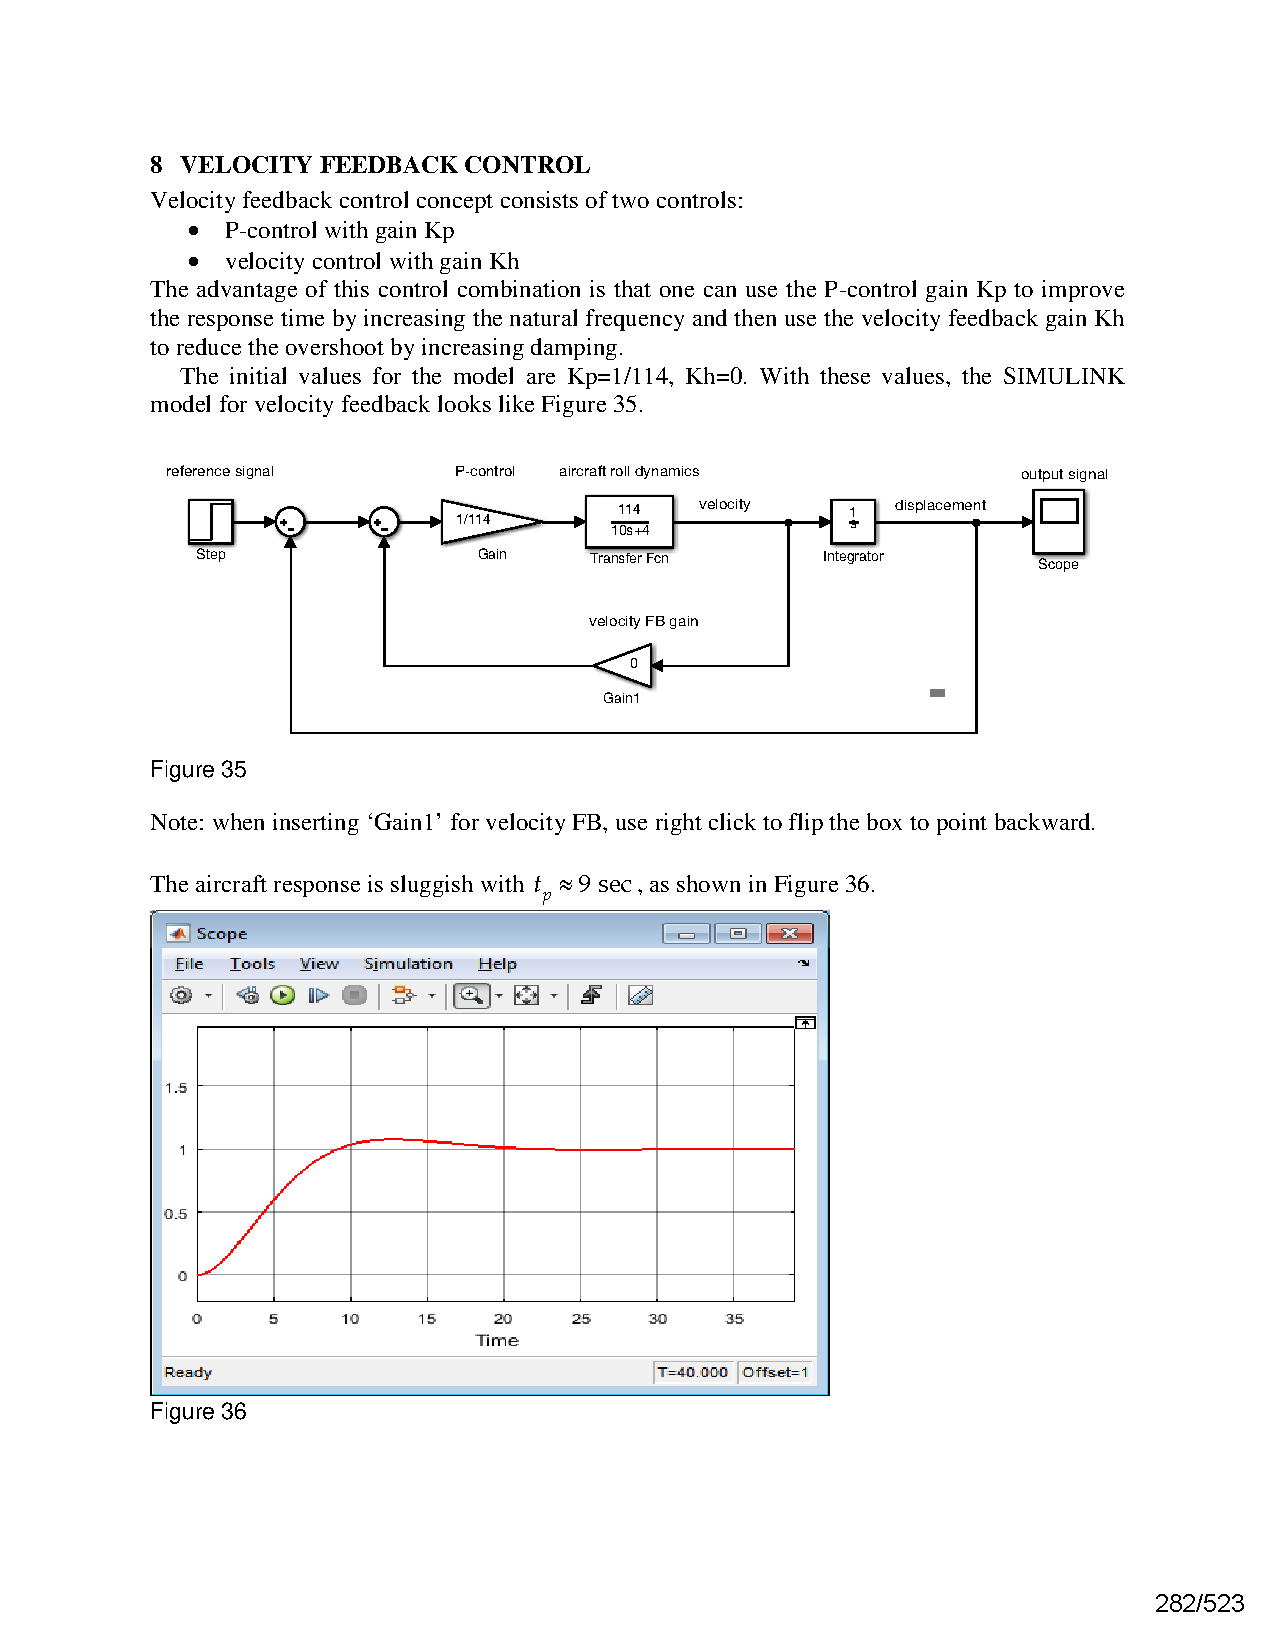
\includepdf[pages=-,pagecommand={},width=0.9\textwidth]{PDF_notes/SIMULINK_Aircraft_Roll_Motion_continued.pdf}

\subsection{Instability Suppression with velocity feedback}
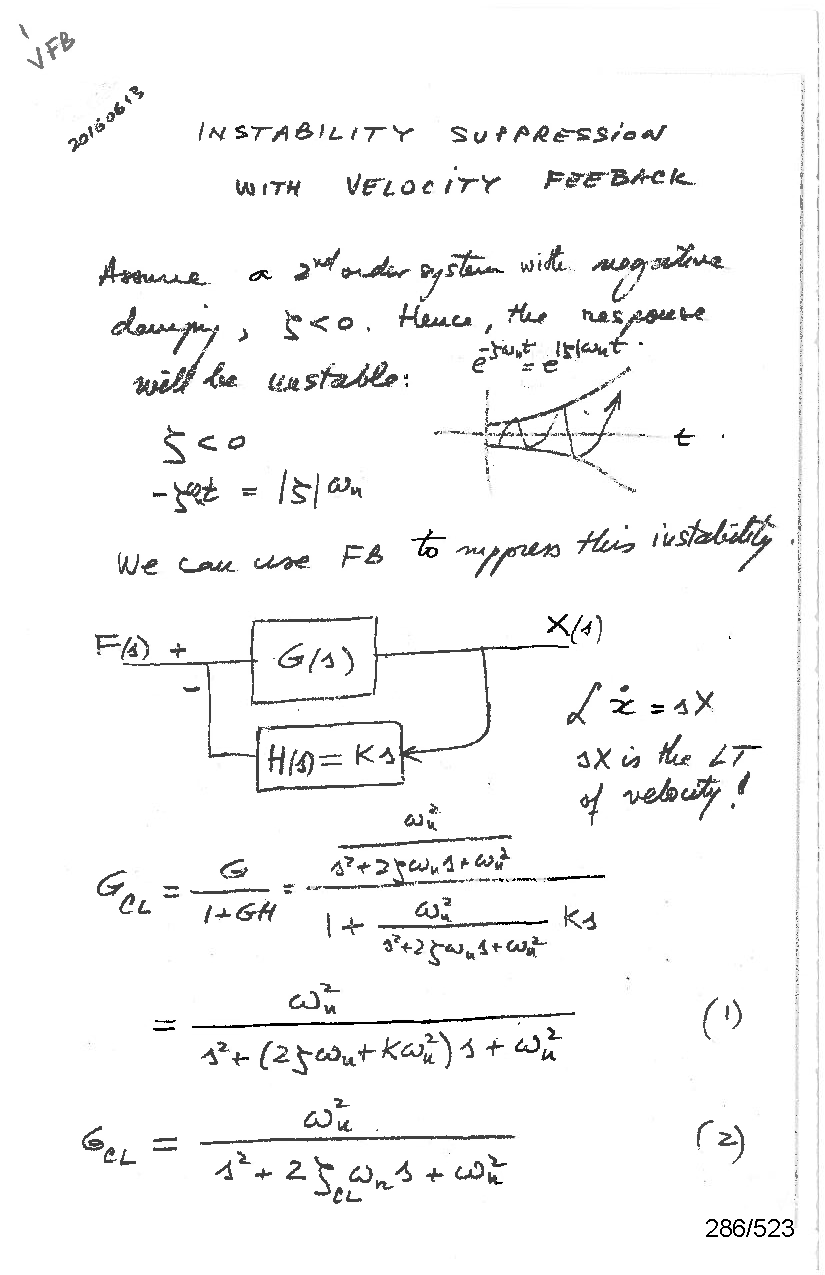
\includepdf[pages=-,pagecommand={},width=0.9\textwidth]{PDF_notes/Instability_Suppression.pdf}



	\pagebreak
	\renewcommand{\thepage}{}
	\renewcommand\refname{References Cited}
	\pagestyle{plain}
	\bibliographystyle{Downey_NSF}
	\bibliography{Chapter_1_Basic_Concepts}


















\end{document}

